\section{Intellectual Merit}
\subsection{Pairwise alignment: Align Pair}
% Talk about pairwise alignment, basis of MSA.

% pair-HMM vs FSTs.
\textbf{Pairwise hidden-Markov models (pair-HMMs)}.
    \begin{itemize}
    \item Computational machine with two output tapes, typically
        a finite-number of states (match, insertion, deletion),
        which emit symbols (nucs, AAs) onto one or both tapes.
    \item A path through the pair-HMM represents the aln between
        the sequences.
    \item Conceptually, a pair-HMM generates two sequences ($X$
        and $Y$) from some unknown common ancestor.
    \item Benefits: rigorously model molecular seq evolution,
        calculate the probability that two seqs are related (Fwd
        algo), estimate optimal aln (Viterbi), and estimate model
        params (Baum-Welsch algo).
    \item Probability of pair-HMM.
        A pair-HMM calculates \parencite{yoon_2009_hmm}:\\
        $P(x,z) = \sum_y P(x,y,z)$
    \end{itemize}

% evolution FST
\textbf{Finite-state transducers (FSTs)}
    \begin{itemize}
    \item Limitation of pair-HMM is that only model evolution of
        two related sequences from an unknown ancestor, and it's
        not possible to use the output of one pair-HMM as ancestor
        of another pair-HMM.
    \item FSTs is similar to a pair-HMM except that it has an input
        tape and an output tape, instead of two output tapes. It
        absorbs symbols from input tape and emits symbols to output.
    \item Conceptually, an FST generates a descendant seq given
        an ancestral one $X \Rightarrow Y$. Properly weighted,
        an FST can calculate the conditional prob that sequence
        $Y$ evolved from seq $X \rightarrow P(y|x)$).
    \end{itemize}

\textbf{Composition}
    \begin{itemize}
    \item FSTs have similar benefits to pair-HMMs + there are
        well established algo for combining FSTs in diff ways
        (e.g. composition: sending output of one FST into input
        of a second one). This allows $P(Z|X) = \sum_Y P(Z|Y) P(Y|X)$,
        represented $X \Rightarrow$ any $Y$ $\Rightarrow Z$.
    \end{itemize}
    \begin{center}
    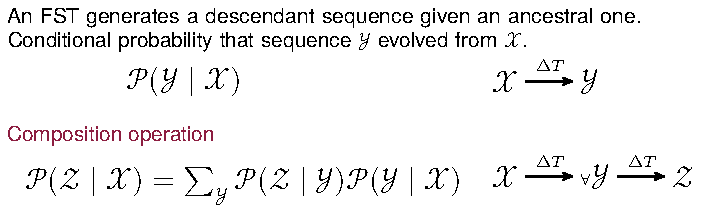
\includegraphics[scale=1]{figures/fig-fst.pdf}
    \end{center}

\textbf{Evolution FST}
    \begin{center}
        \hspace*{-2cm}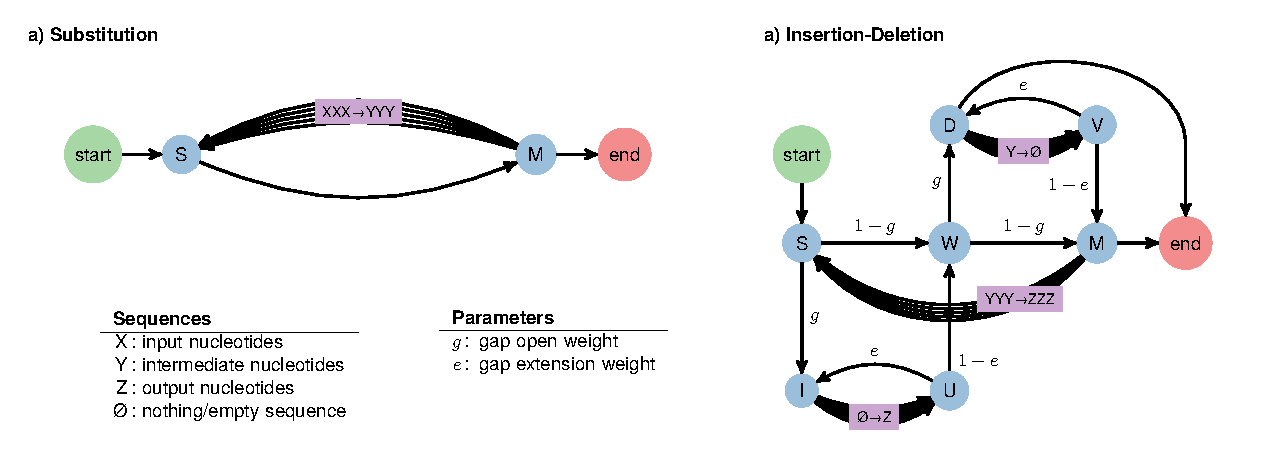
\includegraphics[width=\textwidth]{figures/fig-evolution-fst.pdf}
    \end{center}

% marginalized MG94 codon model
%  justify why we chose that model and what are the benefits/biological implications?

\textbf{MG94 codon model \& marginalization (\red{TODO})}
    \begin{itemize}
    \item MG94
    \item Marginalization
    \end{itemize}

\textbf{Dynamic Programming}
    \begin{center}
        \hspace*{-3cm}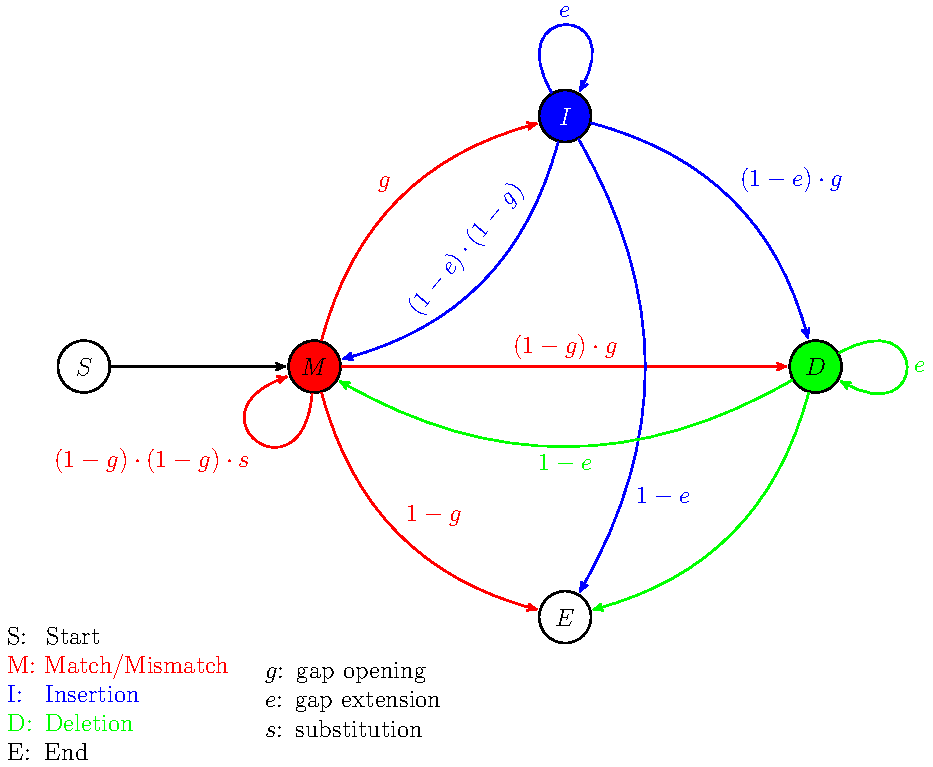
\includegraphics[scale=0.75]{figures/fig-dp-model.pdf}
    \end{center}

% \subsubsection{Ambiguous nucleotides?}
%

% \subsubsection{Stop codons?}
